\chapter{Trasformazioni}\label{trasformazioni}
Una \textbf{trasformazione geometrica} \`e una funzione che mappa punti in punti e vettori in vettori. Quando parliamo
di \emph{trasformazione} di un oggetto intendiamo l'applicazione della stessa trasformazione a tutti i punti
dell'oggetto.

Per semplicit\`a faremo riferimento a punti nello spazio bidimensionale anche se il discorso \`e analogo per punti
tridimensionali.
\[ p = \begin{bmatrix} p_x \\ p_y \end{bmatrix} \]

\section{Traslazione}
La \textbf{traslazione} $T_v$ di un punto $p$ trasla $p$ di un certo vettore $v$.
\[
	T_v(p) = p + v =
	\begin{bmatrix}
		p_x \\ p_y
	\end{bmatrix} +
	\begin{bmatrix}
		v_x \\ v_y
	\end{bmatrix} =
	\begin{bmatrix}
		p_x + v_x \\ p_y + v_y
	\end{bmatrix}
\]
La traslazione \`e indipendente dalle coordinate del punto.

\section{Scalatura}
La \textbf{scalatura} serve a cambiare le dimensioni di un oggetto. Per ottenere questa trasformazione si moltiplicano
tutti i punti della figura per un \textbf{fattore di scalatura}.
\[
	S_{s_x, s_y}(p) =
	\begin{bmatrix}
		s_x \cdot p_x \\
		s_y \cdot p_y
	\end{bmatrix}
\]
Se $s_x = s_y$ allora la scalatura \`e \textbf{uniforme o isotropica} (le proporzioni
dell'oggetto non cambiano). Altrimenti si dice che la scalatura \`e
\textbf{non uniforme o anisotropica}.

\section{Rotazione}
La rotazione $R_\theta$ serve a ruotare di un angolo $\theta$ un punto $p$ rispetto all'origine.

Per effettuare una rotazione abbiamo bisogno di convertire le coordinate cartesiane del nostro punto in coordinate
polari.
\[
	p = \begin{bmatrix}
		p_x \\ p_y
	\end{bmatrix} =
	\begin{bmatrix}
		\rho \cos(\phi) \\
		\rho \sin(\phi)
	\end{bmatrix}\]
Se volessi quindi ruotare il punto $p$ di un angolo $\theta$ rispetto a dove si trova
dovrei svolgere un'operazione di questo tipo:
\[
	R_\theta(p) =
	\begin{bmatrix}
		\rho \cos(\phi + \theta) \\
		\rho \sin(\phi + \theta)
	\end{bmatrix}
\]
Utilizzando le propriet\`a di seno e coseno posso riscrivere la formula in una forma che pi\`u avanti ci sar\`a utile
per svolgere i calcoli pi\`u comodamente.
\begin{gather*}
	\cos(\phi + \theta) = \cos(\phi) \cos(\theta) - \sin(\phi) \sin(\theta) \\
	\sin(\phi + \theta) = \sin(\theta) \cos(\phi) + \sin(\phi) \cos(\theta)
\end{gather*}
Posso quindi riscrivere la funzione di rotazione come
\[
	R_\theta(p) =
	\begin{bmatrix}
		\rho [ \cos(\phi) \cos(\theta) - \sin(\phi) \sin(\theta) ] \\
		\rho [ \sin(\theta) \cos(\phi) + \sin(\phi) \cos(\theta) ]
	\end{bmatrix}
\]
che in forma pi\`u compatta diventa
\[
	R_\theta(p) = \begin{bmatrix}
		p_x \cos(\theta) - p_y \sin(\theta) \\
		p_x \sin(\theta) + p_y \cos(\theta)
	\end{bmatrix}
\]

\section{Taglio}
Il \textbf{taglio} \`e una traslazione di ognuno dei punti lungo un asse in modo proporzionale al valore
dell'altro.
\[
	Sh_{k, y}(p) =
	\begin{bmatrix}
		p_x + k \cdot p_y \\
		p_y
	\end{bmatrix}
\]
Si pu\`o comunque ottenere come combinazione di rotazioni e scalature non uniformi e non \`e molto usata.

\section{Matrice di trasformazione}
Introduciamo ora la cosiddetta \textbf{matrice di trasformazione}. Per ottenerla ci basta accorpare le varie equazioni
che definiscono la trasformazione in un'unica matrice.

Per esempio consideriamo il generico punto $p$ nello spazio bidimensionale. Una generica trasformazione mi far\`a
ottenere il punto $p'$ in questo modo:
\begin{gather*}
	p'_x = a_{xx} p_x + a_{xy} p_y \\
	p'_y = a_{yx} p_x + a_{yy} p_y
\end{gather*}
Dove i vari $a$ sono i coefficienti che dipendono dal tipo di trasformazione che si
vuole applicare.

Posso usare la matrice di trasformazione per scrivere:
\begin{gather*}
	p' = \begin{bmatrix}
		a_{xx} & a_{xy} \\
		a_{yx} & a_{yy}
	\end{bmatrix} \cdot p
\end{gather*}

Precedentemente abbiamo espresso la rotazione di un punto $p$ di un angolo $\theta$
tramite la formula
\[
	R_\theta(p) = \begin{bmatrix}
		p_x \cos(\theta) - p_y \sin(\theta) \\
		p_x \sin(\theta) + p_y \cos(\theta)
	\end{bmatrix}
\]
Da qui ne ricaviamo che la generica \emph{matrice di rotazione} \`e espressa come segue
\[
	R_\theta = \begin{bmatrix}
		\cos(\theta) & -\sin(\theta) \\
		\sin(\theta) & \cos(\theta)
	\end{bmatrix}
\]
Ragionamento analogo per la \emph{matrice di scalatura}, espressa in questo modo
\[
	S_{s_x, s_y} = \begin{bmatrix}
		s_x & 0   \\
		0   & s_y
	\end{bmatrix}
\]
Per quanto riguarda invece la traslazione non \`e cos\`e immediata la conversione dato
che la traslazione non \`e una combinazione lineare delle coordinate (non dipende da dove \`e
il punto), dipende solo dal vettore di traslazione.

Conviene quindi passare alle \textbf{coordinate omogenee}, ovvero si aggiunge un 1 alle
coordinate del punto (se in 2D sar\`a come la terza coordinata, se in 3D sar\`a al posto
della quarta) e uno 0 alle coordinate del vettore.

Se abbiamo ad esempio il punto $p$ e il vettore $v$, entrambi nello spazio bidimensionale,
dovremo considerarli come segue
\[
	p = \begin{bmatrix}
		p_x \\ p_y \\ 1
	\end{bmatrix} \quad
	v = \begin{bmatrix}
		v_x \\ v_y \\ 0
	\end{bmatrix}
\]
Possiamo ora scrivere la nostra \emph{matrice di traslazione} in questo modo
\[
	T_v = \begin{bmatrix}
		1 & 0 & v_x \\
		0 & 1 & v_y \\
		0 & 0 & 1
	\end{bmatrix}
\]
Se vorr\`o applicare la traslazione al punto $p$ dovr\`o moltiplicare tale matrice per il punto
in formato omogeneo.

In generale, ho una \emph{matrice di trasformazione} che posso usare per tutte le trasformazioni
scritta in questo modo:
\[
	\begin{bmatrix}
		a_{xx} & a_{xy} & v_x \\
		a_{yx} & a_{yy} & v_y \\
		0      & 0      & 1
	\end{bmatrix}
\]

\subsection{Composizione di trasformazioni}
Per ottenere effetti diversi e particolari le singole trasformazioni non bastano. Si ricorrer\`a
spesso ad una combinazione di esse, per farlo devo moltiplicare tra loro le matrici di
trasformazione che sto utilizzando.

Se considero ad esempio le tre trasformazioni di base (traslazione, rotazione e scalatura) la
matrice di trasformazione finale sar\`a ottenuta dal prodotto delle matrici associate.
\[ M = T \cdot R \cdot S \]
Se voglio quindi applicare pi\`u trasformazioni al punto $p$, il punto $p'$ sar\`a ottenuto in
questo modo
\[ p' = T \cdot R \cdot S \cdot p \]

\subsubsection{Ordine delle trasformazioni}
L'ordine con il quale si effettuano le moltiplicazioni \`e da tenere di conto. Nella formula vista sopra il punto
$p$ viene prima scalato poi ruotato e infine traslato. Questo perch\'e le trasformazione vengono applicate in ordine
inverso a quello delle moltiplicazioni.

Se avessimo una figura qualsiasi con centro nell'origine e volessimo applicare ad essa una traslazione e una rotazione.
A seconda dell'ordine con il quale vengono applicate le due trasformazioni avremo due effetti molto diversi.

Vediamo un esempio di quanto appena detto usando un quadrato e applicando la
traslazione definita dal vettore $v = \begin{bsmallmatrix} 5 \\ 0 \end{bsmallmatrix}$ e
una rotazione di $\theta = 45^\circ$.
\begin{center}
	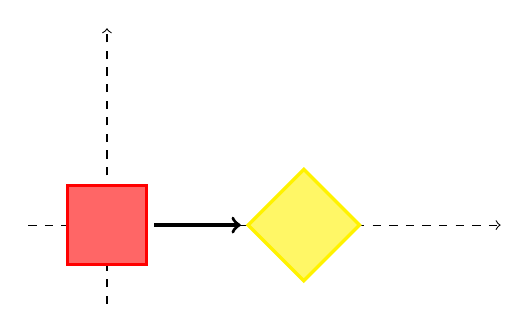
\begin{tikzpicture}[scale=0.5]
		% assi cartesiani
		\draw[dashed](-2,0) -- (0, 0);
		\draw[dashed] (0, -2) -- (0, 0);
		\draw[->, dashed] (0, 0) -- (10, 0);
		\draw[->, dashed] (0, 0) -- (0, 5);
		% prima della trasformazione
		\filldraw[color=red, fill=red!60, very thick]
		(-1, -1) --
		(-1, 1) --
		(1, 1) --
		(1, -1) --
		cycle;
		\draw[color=black, very thick, ->] (1.2, 0) -- (3.4, 0);
		% dopo la trasformazione
		\filldraw[color=yellow, fill=yellow!60, very thick]
		(5, -1.41421) --
		(3.5857, 0) --
		(5, 1.41421) --
		(6.41421, 0) --
		cycle;
	\end{tikzpicture}
\end{center}
In questo caso abbiamo applicato prima una rotazione e poi una traslazione.
\begin{center}
	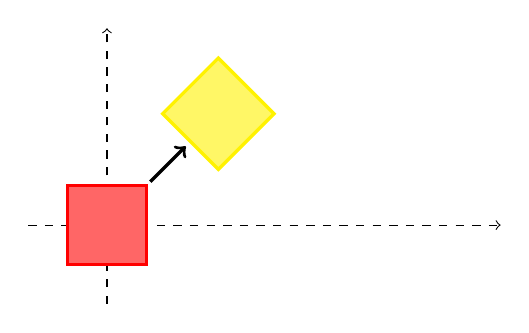
\begin{tikzpicture}[scale=0.5]
		% assi cartesiani
		\draw[dashed] (-2,0) -- (0, 0);
		\draw[dashed] (0, -2) -- (0, 0);
		\draw[->, dashed] (0, 0) -- (10, 0);
		\draw[->, dashed] (0, 0) -- (0, 5);
		% prima della trasformazione
		\filldraw[color=red, fill=red!60, very thick]
		(-1, -1) --
		(-1, 1) --
		(1, 1) --
		(1, -1) --
		cycle;
		\draw[color=black, very thick, ->] (1.1, 1.1) -- (2, 2);
		% dopo la trasformazione
		\filldraw[color=yellow, fill=yellow!60, very thick]
		(2.8284, 1.41421) --
		(1.41421, 2.8284) --
		(2.8284, 4.2426) --
		(4.2426, 2.8284) --
		cycle;
	\end{tikzpicture}
\end{center}
Qui invece abbiamo applicato prima una traslazione e poi una rotazione.

\subsubsection{Cambio del centro di rotazione}
Un caso particolare \`e quello in cui vogliamo far ruotare un oggetto rispetto a un punto
diverso dal centro. Di seguito il procedimento per effettuare questa operazione.
\begin{enumerate}
	\item Individuare il punto intorno al quale effettuare la rotazione.
	\item Traslare la geometria di un vettore tale da portare il punto scelto nell'origine
	      degli assi.
	\item Effettuare la rotazione.
	\item Riportare la figura nella posizione iniziale.
\end{enumerate}

Prendiamo ad esempio un punto $c$ che sar\`a il nostro nuovo centro di rotazione, e prendiamo
un generico angolo $\theta$. Sia $T_c$ la matrice di traslazione che porta $c$ nell'origine,
$R_\theta$ la matrice di rotazione per l'angolo $\theta$ e sia $T_{-c}$ la matrice di
traslazione che riporta $c$ nel punto iniziale, allora per effettuare la rotazione rispetto
a $c$, la matrice di trasformazione che mi serve sar\`a
\[ R_{\theta, c} = T_c \cdot R_\theta \cdot T_{-c} \]
In realt\`a \`e molto pi\`u conveniente usare questa matrice
\[
	R_{\theta, c} = \begin{bmatrix}
		R_\theta & (I - R_\theta) c \\
		0        & 1
	\end{bmatrix}
\]
che se sviluppata \`e sempre una matrice $4 \times 4$.

\section{Trasformazioni affini}
Una trasformazione si dice \textbf{affine} se e solo se:
\begin{itemize}
	\item Preserva la collinearit\`a, ovvero se due o pi\`u punti si trovano su una retta,
	      dopo la trasformazione si troveranno sempre su di una retta (anche diversa da
	      quella iniziale).
	\item Preserva il rapporto tra le distanze tra i punti sulla stessa retta e tra punti su
	      rette parallele.
	\item Preserva il parallelismo tra le rette: se ho insiemi di punti su rette distinte e
	      parallele, dopo la trasformazione si troveranno ancora su rette parallele (anche
	      diverse da quelle di partenza).
\end{itemize}
Traslazione, rotazione e scalatura sono trasformazioni \emph{affini}. Anche una qualsiasi
composizione di trasformazioni affini \`e a sua volta \emph{affine}.

\subsection{Inverso di trasformazioni affini}
Prendiamo la matrice di trasformazione
\[
	A = \begin{bmatrix}
		M & t \\
		0 & 1
	\end{bmatrix}
\]
Dove $M$ \`e la sottomatrice di rotazione e scalatura e dove $t$ \`e il vettore di traslazione.
La matrice inversa di $A$ \`e
\[
	A^{-1} = \begin{bmatrix}
		M & t \\
		0 & 1
	\end{bmatrix}^{-1}
\]
Per le propriet\`a delle matrici sappiamo che
\begin{gather*}
	A A^{-1} = I \\
	(AB)^{-1} = B^{-1} A^{-1}
\end{gather*}
A questo punto possiamo sviluppare l'equazione come segue
\begin{gather*}
	\left(
	\begin{bmatrix}
		I & t \\
		0 & 1
	\end{bmatrix}
	\begin{bmatrix}
		M & 0 \\
		0 & 1
	\end{bmatrix}
	\right)^{-1} \\
	= \begin{bmatrix}
		M & 0 \\
		0 & 1
	\end{bmatrix}^{-1}
	\begin{bmatrix}
		I & t \\
		0 & 1
	\end{bmatrix}^{-1} \\
	= \begin{bmatrix}
		M & 0 \\
		0 & 1
	\end{bmatrix}^{-1}
	\begin{bmatrix}
		I & -t \\
		0 & 1
	\end{bmatrix} \\
	= \begin{bmatrix}
		M^{-1} & -M^{-1}t \\
		0      & 1
	\end{bmatrix}
\end{gather*}
La matrice ottenuta produce una trasformazione inversa a quella di partenza, per esempio se
traslo di un certo vettore $t$, la trasformazione inversa mi fara traslare di un vettore
$-t$.
